%%%%%%%%%%%%%%%%%%%%%part.tex%%%%%%%%%%%%%%%%%%%%%%%%%%%%%%%%%%
% 
% sample part title
%
% Use this file as a template for your own input.
%
%%%%%%%%%%%%%%%%%%%%%%%% Springer %%%%%%%%%%%%%%%%%%%%%%%%%%

\begin{partbacktext}
\part{Muscle Support}
\noindent 
\section*{Muscle Support Overview}

The chapters of Part III are about the supportive environment of the extracellular fluid (ECF). Every chapter describes a set of functions that serve the purpose of delivering, removing or regulating the contents of the ECF. 

Figure \ref{fig:part3_overview} is a graphic overview of the ECF supporting functions. Filtration relies on micro-circulation which relies on circulation. Circulation is the flow of blood through the entire circulatory system. Circulation of blood through the entire body ensures regular mixing of the ECF contents throughout the body. This mixing ensures consistency of ECF contents and a stable environment for all the cells of the body. For example, if blood $Na^+$ concentration is tested, it is properly assumed that concentration is the concentration of $Na^+$ throughout the entire ECF. Circulation also allows each supporting system contribute - either to adding water, heat, ions, molecules or nutrients to the ECF, or removing by-products from the ECF. Supporting systems are also in communication with one another based on the circulating substances and messages (hormones). For example, if a muscle working at high tension is shuttling lactate into the ECF, it is picked up by the circulation and can then enter other cells (heart, liver, non working muscles) where lactate levels are low. In these cells the lactate can be used to produce an $NADH$ from $NAD^+$, and a pyruvate to proceed into the mitochondria. 

\begin{wrapfigure}{R}{0.5\textwidth}
  \begin{center}
   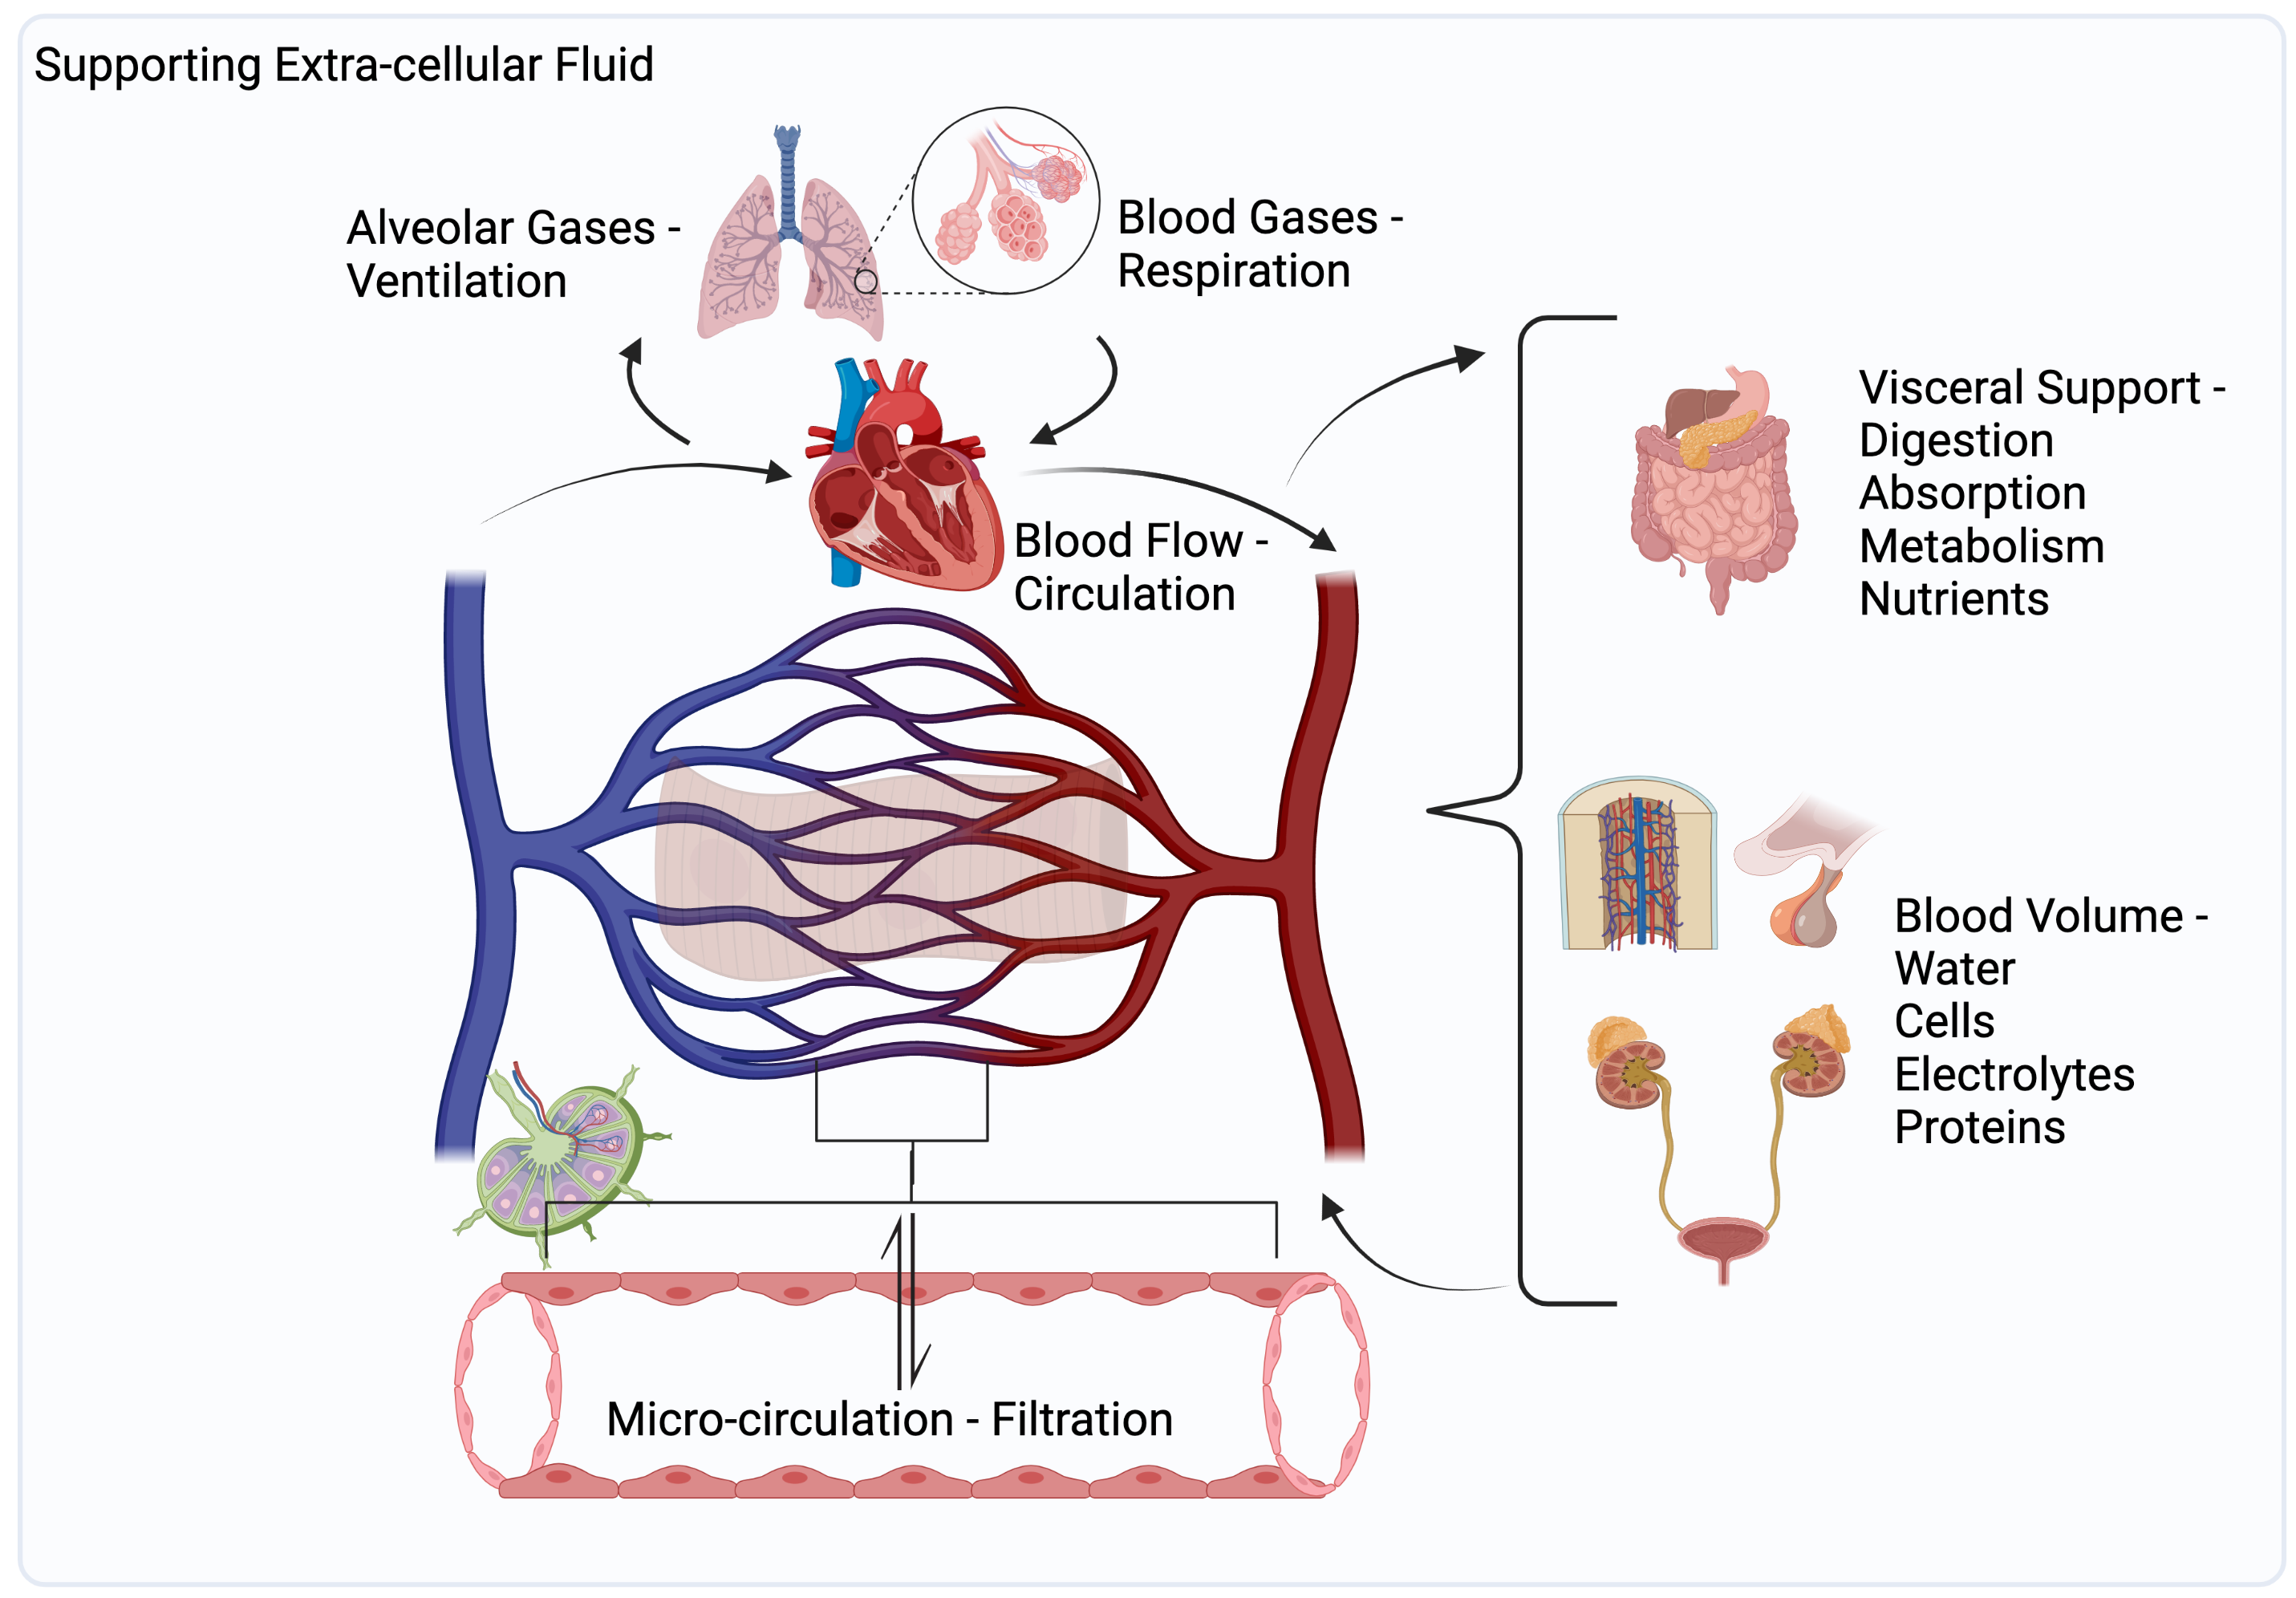
\includegraphics[width=1.0\linewidth]{./figure/part3_overview.png}
  \end{center}
  \caption{Part III: Muscle Support Overview \footnotesize{(Created with BioRender.com)}}
    \label{fig:part3_overview}
\end{wrapfigure}

The contents of blood, and therefore ECF, is regulated and supported by renal filtration (kidneys) and the endocrine system. The regular circulation of blood through the kidneys involves several mechanisms that selectively filter the blood and in doing so regulate the ECF, and therefore the ICF volume. The regulation of fluid volume includes the regulation of several important ions (electrolytes) and the removal of waste (i.e. urea). Working with the endocrine system the kidneys provide long term regulation of blood pressure, which is important for circulation; as well as red blood cells, which is important for oxygen carrying capacity.

Cellular respiration in the mitochondria is constantly using $O_2$ and producing $CO_2$. These molecules are called gases (blood, alveolar) because their natural state is in the gaseous form. The micro circulation ensures the regular delivery ($O_2)$ and removal ($CO_2$) of these gases from the interstitial fluid. The circulation to the lungs ensures the regular exchanges of these gases with the environment. Blood gases rely on blood flow through the lungs for respiration (gas exchange) between the blood and alveoli. Respiration depends on ventilation, the regular movement of these gases into and out of the lungs with the bulk transport of air. 

Maintaining blood nutrients relies on digestion, absorption, metabolism and elimination by the gastrointestinal organs and the liver. Based on the basic physiological concept of mass balance the regular elimination of water requires the regular intake of water. The regular transformation of the carbon bond energy from carbohydrates and fats requires the regular intake of carbohydrates and fat. The regular use, breakdown and elimination of proteins for cellular functions requires the regular intake of protein. 

Together these systems support the ECF and therefore muscle fibers and muscle function. They maintain homeostasis of several important electrolytes (ions, including $H^+$ as measured by pH), nutrients, molecules, water and heat (temperature). The systems are are integrated with several interactions and redundancies to provide support across a wide range of muscle demands in a wide range of circumstances, both good and bad.

One difference between Part II and Part III of the book is that many topics throughout the chapters are in Part III are inherently \textit{Clinical Physiology Connections}. Since the concepts described in Part III are traditional concepts in a clinical physiology course, in many ways these chapters are, in their entirety, clinical physiology connections. As the occasion arises, in pace of \textit{Clinical Physiology Connections} there will be \textit{Muscle Connections}.

\end{partbacktext}